
% This is the main file to setup the document.
% Document organization and appearance settings are all done here
% Each chapter is a separate tex file, all linked together here


% Preamble (document settings) -----------------------------------------------------------
% Document type and font --
\documentclass[12pt,a4paper]{report}
\usepackage[utf8]{inputenc} %utf-8 encoding for ASCII symbols

% insert packages here --
\usepackage{graphicx}       %for handling images

\usepackage{amsmath}        %for math symbols

\usepackage{breakcites}     %to avoid citations extending into the margin
\usepackage{rotating}

\usepackage[margin=1in]{geometry}   %to reduce margins to 1 inch, default margins wasted a lot of space

\usepackage{sidecap}        %to enable side captions on figures

\usepackage{setspace}       %to enable doublespacing

\usepackage[
backend=biber,
style=apa,
citestyle=apa,
maxcitenames=2,
]{biblatex}       %use the biblatex package

\usepackage{float} % for precisely placed float figures https://www.overleaf.com/learn/latex/Positioning_of_Figures

\addbibresource{bibliography.bib}   %path to the bib file

\usepackage{enumitem}


\usepackage{changepage}

\usepackage{hyperref}       % to create a linked table of contents
\hypersetup{
    colorlinks,
    citecolor=black,
    filecolor=black,
    linkcolor=black,
    urlcolor=black
}

% Set path to images
\graphicspath{ {images/} }  % Direct to the main image folder, always good to create sub-folders to organize images for individual chapters

\singlespacing  %making text double spaces

\def\labelitemi{--}

% End of preamble
%-------------------------------------------------------------------------------------------
\begin{document}

% Making title page


\begin{titlepage}
   \begin{center}
   \begin{doublespacing}

       \begin{figure}
       \centering
       
\includegraphics[width=0.7\textwidth]{images/Nanyang_Technological_University.png}
       \end{figure}
       
       
       \vspace{5mm}
       {\large{Progress Report for Confirmation of Candidature}\\
       {to the degree of Masters of Engineering}}

       \vspace{30mm}
       
       {\Large\textbf{A Scalable Multi-Constraint Approach to Automating Teaching Workload Allocation}}
       
%        Automating Workload-Aware Teaching Allocation

    
            
       \vspace{20mm}
       
       by
       
       \vspace{20mm}

       {\Large\textbf{Arpit Roopchandani}\\
       {G2004728A}}

       \vfill
       {\large \textbf{School of Computer Science and Engineering}\\
       \textbf{March, 2022}}
       
    \end{doublespacing}

   \end{center}
\end{titlepage}


% Starting frontmatter:
% Abstract goes here
\doublespacing

\begin{abstract}

  Faculty workload allocation and scheduling are key factors contributing to the quality of research, teaching and service in large educational institutions. This necessitates the development of suitable workload models for research, teaching and service to facilitate the equitable distribution of workload among research-active faculty. In this research work, a suitable workload model for evaluating the research workload of a faculty has been proposed based on the attributes of the research group of a faculty. Teaching workload model relies on formal and informal teaching components as well as weighted association among lectures, tutorials, and labs. A novel technique for accommodating large class sizes based on available teaching expertise has also been proposed. The main aim of this research is to realize an automated teaching allocation system that can incorporate faculty preferences and teaching priorities to achieve an inclusive, transparent, and objective distribution of teaching workloads while improving the overall faculty satisfaction levels.

\end{abstract}

\pagenumbering{roman}   % Roman page numbering to start from abstract onwards
\addcontentsline{toc}{section}{\textbf{Abstract}}
\listoffigures          % generate list of figures
\singlespacing          % keep pre-content single spaced
\addcontentsline{toc}{section}{\textbf{List of Figures}}
\listoftables           % generate list of tables
\addcontentsline{toc}{section}{\textbf{List of Tables}}

% End of frontmatter

% Insert table of contents
\tableofcontents


% Main matter starts here --
% Inserting individual chapters. Mention chapter titles here and simple link the chapter's tex file
\doublespacing

\chapter{Introduction}
\pagenumbering{arabic}    % We want Arabic numerals for main matter page numbering
\chapter{Introduction}

This chapter briefly introduces the problem of holistic teaching workload allocation in research-intensive universities. It also describes the structure of the report and the contents of its corresponding chapters.

\section{Background and Motivation}

Teaching workload allocation and scheduling are some of the most crucial activities in educational institutions of all sizes. Although done once every semester, this activity forms the backbone of the university environment and governs how much time faculty members can spend in individual areas of the workload like preparing for lectures, delivering lectures, spending time on research and administrative work. Thus, it has a drastic impact on the academic performance of students, the quality of teaching, and the research outputs of the university.

In addition, the teaching workload allocation process is also a key factor in determining the satisfaction of faculty members. A good allocation process ensures that faculty members are allocated courses that they are interested in teaching and that they are allocated a fair amount of workload. This is especially important in research-intensive universities, where faculty members are expected to spend a significant amount of time on research. A good allocation process also ensures that faculty members are not overburdened with workload, which can lead to burnout and dissatisfaction. Additionally, it recognizes the fact that faculty members have different workload patterns and equitably distributes the workload among them.

Historically, this problem has been difficult to automate due to the various conflicting factors that govern the allocations, the massive scale of the problem in large universities, and difficulties in accurately quantifying the workload of faculty members. If done poorly, the allocation can lead to faculty dissatisfaction and inefficient usage of the precious time of students, faculty, and administrative staff.

This is a problem that has typically been solved manually with the help of spreadsheets and other tools. However, as the number of faculty members and courses increases, this process becomes increasingly difficult to manage, resulting in weeks of planning and manual effort to allocate the workload. Even with this considerable effort, it leads to a nearly static allocation that is carried forward from previous years. This leads to a lack of variety in the teaching schedule of faculty members, and an ever-increasing workload for some faculty members, while others are underutilized. This also makes it difficult to make changes to the curriculum, as the allocation is not flexible enough to accommodate these changes.

Although there are multiple in-house techniques and existing solutions to solve this problem, this problem is under-explored, every university has its own unique requirements, and there is no one-size-fits-all solution. Additionally, there are problems with workload inequity and faculty dissatisfaction which, although studied as a separate problem, are not considered holistically in the automated teaching allocation processes.

In this research exercise, we aim to explore the problem of teaching workload allocation in research-intensive universities and propose a solution that can be used to allocate teaching workload fairly and equitably, while also taking into account the preferences of faculty members and the requirements of the university.

\section{Research Objectives}

The primary objective of this research is to develop a holistic teaching workload allocation system that can be used to allocate teaching workload fairly and equitably. This should account for the student feedback on the quality of teaching, the preferences of faculty members, management requirements, and the workload of faculty members in other areas like research and administration.

In the process of developing this system, we also aim to develop a model to accurately quantify the workload of faculty members in non-teaching areas like research and administration. This model should then be able to provide an accurate representation of the various workload constituents of faculty members, which can then be used to allocate teaching workload fairly and equitably.

\section{Organization of the Report}

In this chapter, we discussed the motivation behind the development of a holistic teaching workload allocation system. We also discussed the objectives that we aim to achieve through this research exercise.

\textbf{Chapter 2} offers an overview of existing research and solutions in the area of teaching workload allocation. This includes research into the problems with existing allocation systems, various methods of quantifying and modeling faculty workload, existing solutions to the problem of teaching workload allocation, and other algorithms that are applicable to allocation problems in general. We then discuss the gaps in existing research and how this research aims to fill those gaps.

\textbf{Chapter 3} describes the process of quantifying the teaching workload of faculty members. This involves dividing the workload into various constituents, and then for each constituent, defining the various factors that affect the workload. It then describes the process of quantifying the workload for each constituent to arrive at the total workload for a course. It also describes a lecture-splitting methodology, which is used to split high-workload lectures into smaller pieces, and aims at reducing the workload of faculty members.

\textbf{Chapter 4} describes the process of modeling the workload of faculty members in non-teaching areas like research and administration. This involves identifying the challenges in quantifying the research workload, before defining a technique to quantify the research workload. It then describes the process of quantifying service workload, before describing the process of combining the workload in all areas to arrive at a workload model that describes the workload constitution of faculty members. This workload model is then used to determine the equitable teaching workload for faculty members.

\textbf{Chapter 5} describes the process of allocating lectures to faculty members. To achieve this, it first defines what constitutes a good allocation, and then describes the process of modeling the allocation problem and using the Hungarian algorithm to solve it. Building on this, it adds additional constraints to avoid overloading faculty members and then describes the process of resolving unallocated courses. It then describes the process of equitably overloading faculty members to ensure that all courses are allocated.

\textbf{Chapter 6} describes the process of allocating tutorials and labs to faculty members. It first describes the process of modeling the allocation problem and using the Hungarian algorithm to solve it. It then describes improvements to the cost function to ensure that various requirements are met. It also describes the process of batch allocation of tutorials and labs and the process of dynamically adjusting workload limits to ensure that the allocation is feasible. It then combines all these processes to describe the tutorial and lab allocation process. Finally, it describes the results of the allocation process and the impact of various parameters on the allocation process.

\textbf{Chapter 7} concludes the report by summarizing the research and its findings. It also describes the future work that can be done to improve the allocation process and the research.
 % Link to the chapter tex file

\chapter{Literature review}
\chapter{Literature review}

\section{Introduction}

The course allocation process is a complex process that involves multiple stakeholders, each with their own set of expectations. The key stakeholders are the faculty, the students, and the management. The faculty expects a fair allocation of courses that aligns with their research interests and teaching preferences. The students expect the best possible teaching experience, with faculty that have good feedback in the past. The management expects a optimal utilization of faculty, and to ensure the long term learning outcomes of the students are met.

The allocation process has various prerequisites that need to be provided for the allocation to be effective. The course allocation process can be divided into multiple different sub-problems, each with their own set of objectives and constraints. These sub-problems are:

\begin{enumerate}
  \item \textbf{Course Workload Modelling}

        The first step in the allocation process is to quantify the workload that is involved in teaching a course. This involves quantifying the time required for each of the activities involved in teaching a course. This is a key step in the allocation process, as it provides a clear picture of the workload involved in teaching a course. This is critical in ensuring that the faculty is not overloaded with courses, and that the faculty is not under-utilized.

  \item \textbf{Workload Distribution}

        The next step in the allocation process is to distribute the workload among the faculty. This involves quantifying the non-teaching aspects of their workload like Research and Service, and then distributing the teaching workload among the faculty based on their non-teaching workload. This is a key step in the allocation process, as it ensures that the distribution of the teaching workload is fair and equitable.

  \item \textbf{Allocation}

        The final step in the allocation process is to allocate the courses to the faculty. This involves taking into account the preferences of the faculty and the student feedback, and then allocating the courses to the faculty. This also involves taking into account the constraints of the faculty, like the amount of workload they can handle, while ensuring optimal utilization of the faculty. This allocates the lectures, tutorials, and labs to the faculty.

\end{enumerate}

In this literature review, we will look into the existing approaches to each of these sub-problems, and identify the key issues with the existing approaches. We will look into the existing models of quantifying the workload involved in teaching a course, and identify the key issues with the existing models. We will also look into the existing approaches to distributing the workload among the faculty. Finally, we will look into the existing approaches to allocating the courses to the faculty, as well as the existing algorithms for allocation problems, and their applicability to the course allocation problem. We will also look into the basis of the allocation priorities that are used in the allocation process.

\section{Quantifying Course Workload}

A systematic review on burnout of university teaching staff by \textit{Watts et al.} \cite{watts2011burnout} identified various factors that contribute to burnout of university teaching staff, including the necessity to teach large volume of students with bad student-staff ratios. \textit{Jensen et al.} identified that staff not being given adequate time to account for the preparation and marking of courses was a key problem unrecognized by the management, which led to undue stress for the faculty members \cite{jensen2009vanishing}.

In a case study for the development of a quantifiable academic workload model, \textit{Kenny et al.} state that a lack of clarity about how to quantify academic workload leads to deterioration of academic performance\cite{kenny2012placing}. They also stated that the nature and extent of academic work must be accounted for in a credible and transparent way, and that allocation of workload should account for these factors.

\textit{Houston et al.} \cite{houston2006academic} argued that the diversity of academic work makes it difficult to arrive at a clear standardised quantification of academic workload. However, several attempts have since been made to quantify the academic workload. \textit{Vardi} \cite{vardi2009impacts} broadly categorizes existing workload models into three categories:

\begin{enumerate}

  \item \textbf{Contact Hours based}

        This is a time-based approach used to standardize teaching commitments, relying on typical values without accounting for the nature of the contact, such as lectures, tutorials, or labs, or other variables like class size or course novelty. This model includes standardized additions for tasks like preparation and assessment, and administrators may provide additional support for factors like class size outside of this system. Its aim is to maintain relative fairness among staff through a straightforward system. While effective when teaching expectations are reasonable and allowances for supplementary activities are possible, it struggles to incorporate non-direct duties like research, community work, and clinical trials. These models primarily consider the time needed for course-related tasks and make fixed allowances for associated activities but overlook crucial elements like class size or a faculty member's familiarity with the course.

  \item \textbf{Actual Hours based}

        The 'Actual hours' model is a more detailed time-based approach that takes into account the specific nature of a faculty member's activities. These models strive to cover all facets of a faculty's workload by estimating the time required for each task. For example, they consider the type of assessment and the number of students for marking tasks, as well as the time spent in student consultations and responding to emails. This results in a comprehensive system that aligns more closely with human resourcing and costing. Yet, these approaches tend to be ad-hoc and demand significant effort to accurately model each faculty member's workload.  However, its complexity reduces transparency, leading some faculty members to perceive it as a sign of distrust from the administrators. Additionally, they are viewed as micromanaging, being overly prescriptive about the exact amount of time allocated to each activity. This perception stems from their granular approach to time allocation, which may feel restrictive to faculty members.

  \item \textbf{Points based}

        The 'Points model' is an alternative method for quantifying workload, using a system that converts various faculty activities into 'points', loosely based on the hours of effort required. Faculty members accrue points for different tasks, but this system has been deemed the least effective by both faculty and administrators. Similar in concept to actual-hours models, although the Points model offers some flexibility in time allocation for respective tasks, Faculty members criticize the vague correlation between 'hours' and 'points', alongside a perceived bias favouring activities with greater financial or budgetary returns, highlighting a disconnect between the model's metrics and the diverse responsibilities of faculty members. Administrators find the model inadequate in identifying faculty who are overburdened or underutilized, and are concerned about the neglect of activities that don't earn points.
\end{enumerate}


\textit{Vardi} stated that while a simple model is highly desirable for ease of use, it is important to ensure that the model is not too simple to be ineffective. The model has to account for the variance and complexity of the academic workload among different faculty, and a simple model would fail to do so \cite{vardi2009impacts}.

\textit{Griffith et al.} \cite{griffith2020framework} proposed a framework for quantifying the course workload which divides the teaching workload into three parts - classroom workload ($T_c$), administrative workload ($T_a$), and preparation workload ($T_p$). ($T_c$) is calculated by the total number of hours spent in the classroom and labs per week multiplied by the number of weeks that teaching is required during the contracted period. ($T_a$) is approximated by multiplying the total number of semester credits taught as prescribed by payroll purposes during the contracted period by the 16 weeks in a typical semester. ($T_p$) is estimated by the number of unique courses taught in a contracted period multiplied by four weekly hours and then multiplied by the number of semester credit hours assigned to each course.

\subsection{Limitations of current methods}

\textit{Jensen et al.} mentioned the lack of time being provided for marking of courses, and preparation of courses \cite{jensen2009vanishing}. This led to faculty investing their personal time to mark courses, and felt under-recognized for the time and effort they put into the preparation of contemporary, quality course material. This is a key issue with the contact hour based approach, as it fails to account for the time spent on these activities.

The actual hours approach has issues with effectiveness, due to difficulties in enforcing the model. The key reason being the need to accurately quantify the time spent on a plethora of activities in the form of hours, some of which are not directly measurable \cite{kenny2014effectiveness}. This leads to ambiguity and a case by case approach to workload allocation, which is not scalable and leads to lack of transparency.

In a 2021 study on the emerging state of workload allocation \cite{kenny2021emerging}, Kenny et al. identify that the workload allocation's inability to identify key tasks involved in teaching, such as preparation and marking of courses was stated as the primary challenge towards a fair workload allocation.  This emphasizes a need for a more comprehensive quantification of course workload that accounts for all the activities involved in teaching.

While the approach used by \textit{Griffith et al.} provides a comprehensive view of the teaching workload, it also fails to account for class size, course newness, and faculty familiarity with the course. However, the division of teaching workload into three parts - classroom workload ($T_c$), administrative workload ($T_a$), and preparation workload ($T_p$) is a key step in the right direction, as it provides a clear picture of the workload involved in teaching a course, and indicates towards the impact of different factors to each of these constituents.

None of the models incorporate several important factors. Class size i.e. the number of students in a class which will have a proportional impact on the marking workload for a course, since every student needs to be marked separately - the work required for marking the exams of a course with 30 students is significantly less than that of a course with 300 students. It also needs to be considered whether new material needs to be developed for the class, and the faculty's familiarity with the course, since preparation of a new course adds a significant burden to the faculty. These factors are critical in determining the amount of time required for teaching a course. \textit{Lowenthal et al.} \cite{lowenthal2019does} also clearly identified the impact of class size on the workload, with 75.7\% of the faculty stating that class size has an impact on the workload.

Several of the models were also retrospective in nature and aimed at surveying and quantifying the workload of the faculty in the previous year. However, for the purposes of workload allocation, it is important to quantify the workload of the faculty in the upcoming year, which might not be the same as the previous year. As a result, the workload model needs to be prospective in nature, and should be able to quantify the workload of the faculty in the upcoming year as a function of the factors involved, which was only solved by \textit{Griffith et al.} \cite{griffith2020framework}.

Overall, due to the lack of a comprehensive workload model that accounts for all factors, the need for a new workload model that accounts for all the teaching activities involved, while accounting for class size, course newness and faculty familiarity is felt.

\section{Workload Models}

There are several key steps to allocating teaching workload to the faculty. The first step is to quantify the workload involved in teaching a course. The second step is to identify the non-teaching workload of the faculty, which includes research and service workload. Using these two, the teaching workload of the faculty is calculated. In this section, we will look into the existing approaches to quantifying the research and service workload of the faculty.

Additionally, some of the existing research looks into workload models, which aim to provide a framework for quantifying and distributing the workload among the faculty. Some of these models are discussed in the following sections, along with the shortcomings and scope of improvement for these models.

\subsection{Research and Service Workload}

The working life of a university faculty comprises primarily three parts - Service, Research, and Teaching. Each university has a different set of expectations from the faculty in each of these areas, but broadly speaking, the contributions towards furthering the university's research outputs is considered as Research Workload, and all other workload except from Teaching and Research is considered as Service Workload. This includes administrative duties, community service, and other activities that are not directly related to teaching or research.

The simplest solution to equal distribution of workload between faculties (or equal misery) in all three areas \cite{gray1989university}. However, as different faculties do not display an equal affinity or competency towards these areas \cite{finlay1994management}, equal distribution would lead to inefficient use of the faculties' skill-sets. Additionally, \textit{Deem et al.} \cite{deem2020new} identified that placing pressures on academic staff to increase their number of publications is viewed unfavourably, as it leads to a focus on quantity over quality. This is a key issue with the research workload, as it is difficult to quantify. Moreover, it is seen that research-active faculty ends up doing more research at the cost of overloading and diminishing the quality of teaching.

\textit{R. Sood} \cite{rohan2017} proposed a novel approach to quantifying the research workload, by treating the number of research staff supervised by a faculty as a proxy for the research workload. This is a key step in the right direction, as it provides a clear picture of the research workload of the faculty. However, an analysis of the research workload of faculty showed that beyond a point, economies of scale that are achieved due to the inherent hierarchical nature of research supervision, with the faculty supervising a few senior researchers, who in turn supervise a few junior researchers. Thus, additional considerations need to be made to account for these economies of scale.

\cite{rohan2017} proposed an approach of treating research and service workloads in directly relaxing the teaching workload expectations from a faculty. However, even though the teaching workload relaxation approach works great in practice for allocating teaching workload, it fails to provide a clear picture of the workload distribution among the faculty. This is because the teaching workload relaxation approach is a reactive approach, and does not aim to analyze the workload distribution among the faculty.

The STAR Model (Service, Teaching, Administration, Research) proposed by \cite{finlay1994management} was a key stepping stone in defining the non-teaching parts of a faculty's workload. It focused more on allocating research time as a function of the other three activities. However, the approaches towards calculating each of the constituents were not provided, and the model was not widely adopted. \textit{Burgess et al.} found that a simpler TRO - Teaching, Research, and Other model was preferred by faculty \cite{burgess2003academic} because of its contemporary nature and official sanction in the Transparency Review.

\begin{equation}
  T_c + T_a + T_p + S_i + S_p + S_c+R = C
  \label{griffith_wam}
\end{equation}

Recently, \textit{Griffith et al.} goes much further in describing the constituents of Service Workload as \textbf{Professional}, and \textbf{Community} Service Workload (\(S_p, S_c\)), and the constituents of Teaching workload as \textbf{Classroom}, \textbf{Administrative} and \textbf{Preparation} Teaching Workload (\(T_c, T_a, T_p\)) as shown in \autoref{griffith_wam} \cite{griffith2020framework}. This provides much needed clarity into the nature of the work involved in each of these constituents. It also highlights key problems the academic community faces in each of the workload constituents. However, it omits the inclusion of faculty-specific deviations to the teaching workload and the variation in workload depending on the faculty type. Additionally, it doesn't provide a framework for quantifying the research workload and the service workload of the faculty.

In a 2021 journal, \textit{Narasimhan et al.} explored a new TRASE model, accounting for Teaching, Research, Administration, Service, and Entrepreneurship \cite{narasimhan32trase}. This provided a workload factor for each of the constituents, given for a level of participation and workload in each of the constituents. "if a person wants to have a teaching load of 30\%, research load of 50\% and service load of 20\%, then s/he has to have: i) two subjects per semester, ii) three conference papers or 1-3 journal papers per year with one paper in Tier-I level and obtain funding to the tune of 4,00,000/year and have two PhD/MS students and iii) participate in 2 committees and perform at least one other significant activity."

\subsection{Issues with current workload models}

\textit{Doyle et al.} and \textit{Winefield et al} reported time pressures and lack of time for research \cite{doyle1998occupational,winefield2003occupational}. This was also reported by \textit{Jensen et al.} \cite{jensen2009vanishing}, who identified that the lack of time for research was a key factor in the burnout of faculty.

However, it was found that although there exist several approaches to quantifying the teaching workload, there is a lack of approaches to quantifying the research workload and the service workload. Additionally, most of the proposed approaches to quantifying various types of workload fail to bring them to a common scale, which makes it difficult to compare the workload of different faculty. Burgess \cite{burgess2003academic} stated that transparency in workload allocation is critical to ensure wider acceptance of the workload model by the faculty members.

Thus, the need for a comprehensive workload model that accounts for all the teaching activities, as well as the research and service workload, was felt. This workload model should also be able to quantify the workload of the faculty on a common scale to allow for comparison of the workload of different faculty. \textit{Kenny et al.} \cite{kenny2021emerging} identified issues with the workload allocation processes to identify and equitably account for the key tasks involved in the faculty workload. A comprehensive workload model can help highlight the distribution of workload among the key areas and improve visibility of staff workload.

Overall, the key issues with the existing WAMs can be summarized as follows:

\begin{enumerate}

  \item \textbf{Inability to accurately quantify research workload}

        Most WAMs do not account for the research workload. The few models that quantify the research aim to do so using the research output. However, these approaches assume an equal amount of time required for different research work and, thus, fail to account for the varying amounts of time different research activities require. It's also dangerous to base teaching output on the number of publications, since it incentivizes quantity over quality. In this regard, the approach adopted by \textit{R. Sood} \cite{rohan2017} had merit, as it quantified the research workload as a function of the number of research staff supervised by a faculty which is difficult to abuse, because hiring additional research staff is expensive.

  \item \textbf{Teaching Centric}

        Various models were Teaching Centric, and fail to give a clear picture of the workload distribution by treating service and research workloads as concessions to teaching, and thus fail to provide organizational insights into the overall workload distribution. \cite{rohan2017}. Since the final output of such models is the teaching workload, it leads to a lack of transparency in the workload distribution among the faculty, and thus may lead to lack of acceptance of the workload model by the faculty.

  \item \textbf{Lack of organizational insights}

        Various approaches attempting to quantify the areas of workload also fail to bring them to a common scale, which makes it difficult to compare the workload of different faculty. Seeing each of the areas of workload as a separate entity may result in the management's failure to recognize the areas of workload that are classically prone to overload, such as research and service. This may lead to the management's lack of organizational insights into the workload distribution among the faculty. The TRASE model \cite{narasimhan32trase} is a step in the right direction, putting all the constituents of workload on a common scale.

  \item \textbf{Retrospective approach}

        Of the few models that manage to quantify the research workload, most are retrospective in nature and have an inability to account for unpublished research. This leads to inaccuracies, since the rewards for research are retrospective and don't reflect the current workload. eventually align to a Garbage-In-Garbage-Out due to their dependence on research output. This ensures that the current year will only be able to reach a research output similar to the previous year due to a proportional amount of teaching work allocated in this year. Additionally, it causes issues with periodicity. For example, in the worst case, looking at the research output of a faculty in the fall semester might seem high due to major conferences being held in that period, which will reduce their workload for spring semester, but lack of research output in the spring semester might lead to a high workload in the fall semester, which is undesirable.

\end{enumerate}

\subsection{Workload Inequity as a systemic problem}

\textit{Jensen et al.} \cite{jensen2009overload} and \textit{Kenny et al.} \cite{jensen2009overload, kenny2014effectiveness} identify that workload modelling and distribution fails to make an impact due to the lack of additional resources made available to address workload inequities. The lack of available expertise in key areas disproportionately overloads certain faculty with said expertise, essentially punishing faculty for being skilled.

\cite{vardi2009impacts, houston2006academic} clearly identify that even with the mandated use of WAMs in Australian universities, overloading of faculty is a widespread problem due to under-supply issues.\cite{kenny2014effectiveness} also notes that defining realistic time limits is a necessary step towards ensuring welfare of academic staff. One of the big reasons for this was identified as budgetary concerns, with universities being unwilling to hire additional faculty to address the workload inequity \cite{kenny2012placing}.

This is a key issue with the workload allocation, as workload inequity is a systemic problem that cannot be solved by the workload allocation process alone. In the absence of additional resources, the best the workload allocation process can do is to ensure that the workload is distributed equitably among the faculty, overloading them on an equitable basis. However, it was found that this is not a sustainable solution, as it leads to faculty burnout and attrition.

\section{Allocation Priorities}

\cite{harwood1975optimizing} identifies the three key stakeholders of workload allocation as the faculty, the students, and the administration. The faculty expects a fair allocation of courses that aligns with their research interests. The students expect a variety of courses that allows them to customize their academic journey, and expect the best possible teaching experience, with faculty that have good feedback in the past. The administration expects a optimal utilization of faculty, but are largely in alignment with the faculty and student expectations.

\textit{Schniederjans et al.} and \textit{Badri et al.} \cite{schniederjans1987goal, badri1998multi} further go into the role faculty preferences play in this distribution, with the faculty being able to express their preferences for the courses they want to teach.

\textit{R. Sood} \cite{rohan2017} identified another management priority - the need to ensure that the best faculty are allocated to earlier year courses, which are critical in setting the foundation for the students' academic journey. This is a key priority, as it ensures that the students get the right amount of guidance in the early years, while they gain more autonomy and independence in the later years, and build the skills to self-learn. Additionally, a bias was identified towards allocating faculty to courses they have taught in the past, as they are familiar with the course material and the teaching style, and thus require less work to prepare for the course.

With this in mind, the following allocation priorities were identified:

\begin{enumerate}
  \item Faculty

        — Faculty course preferences are important as they allow them to align their teaching with their areas of research interest

        — Faculty should be allocated to courses that they have taught in the past, as they are familiar with the course material and the teaching style, and thus require less work to prepare for the course

        — Schedule preferences also allow them to create windows in their schedule for focused research and administrative work that fits their work styles

        — Faculty should not be overloaded with courses, as it leads to lack of time towards research, which is important for their career progression

  \item Student Body

        — Students expect a minimum variety of courses that allows them to customize their academic journey

        — Students expect the best possible teaching experience, with faculty that have good feedback in the past

  \item Administration

        — Maintain equitable distribution of work among the staff and lack of bias

        — Ensure that the best faculty are allocated to earlier year courses, which are critical in setting the foundation for the students' academic journey

        — Ensure optimal utilization of faculty

        — Ensure that the faculty are not overloaded with courses, as it leads to burnout and attrition

\end{enumerate}

These priorities establish a good basis for the allocation process, providing the key objectives and constraints for the allocation process. There is a need to mathematically quantify these priorities to allow for allocation algorithms to use them as a basis for the allocation process. Additionally, a prioritization needs be defined for these objectives and constraints, as they are not of equal importance. For example, the need to ensure that the faculty are not overloaded with courses is more important than ensuring their preferences are met.

\section{Existing Approaches to Course Allocation}

\textit{Schniederjans et al.} \cite{schniederjans1987goal} originally proposed a goal-programming algorithm for solving a preference-aware course allocation algorithm. This was a good approach that resulted in balanced assignments that aim to satisfy the requirements of both the department, and the faculty preferences. Although much more efficient than the traditional subjective approaches however, it fails to apply on large-scale universities due to its high time complexity due to its matrix optimization methodology. Additionally, the high complexity of the model makes it difficult to implement, especially in departments with a large number of faculty members and courses.

\textit{Sood R.} \cite{rohan2017} opted for a greedy solution due to the massive complexity involved in expressing a many-to-many allocation with multiple levels of course-priority in a goal-programming solution. The greedy solution involved iterating through the courses and allocating the best faculty available. The solutions produced by this approach were observed to be satisfactory, but had a tendency to converge local minima. This was countered using an Iterated Greedy algorithm inspired by the \cite{ruiz2007simple}, which goes through multiple phases of random destruction and reconstruction of the solution to converge towards a better solution. However, the inherent greediness of allocating courses one-at-a-time leads to sub-optimal solutions, as it fails to account for the inter-dependencies between courses.

\textit{Sood R.} also explored the application of the Kuhn-Munkres algorithm, commonly known as the Hungarian algorithm, to allocating Student Final-Year Projects. However, this wasn't explored for the course allocation problem \cite{rohan2017}. It is also important to note that the Hungarian Algorithm \cite{munkres1957algorithms} is the go-to algorithm for one-to-one matrix-optimization problems, but it fails to directly apply to many-to-many solutions with inter-dependent allocations. Hence, great care needs to be taken to orchestrate the many-to-many allocation problem into a one-to-one matrix-optimization problem.

\textit{Mallicka et al.} \cite{mallicka2021claps} explored the application of the Hungarian algorithm to build a "Course and Lecture Assignment Problem Solver". For this, the considerations include faculty expertise, effectiveness in course delivery, and the goal of minimizing preparation time while maximizing teaching effectiveness. It failed to address the problem of many-to-many allocations, and thus remains limited to an idealistic one-to-one allocation problem. Additionally, it relied on a self-rated effectiveness score, which is subjective and difficult to quantify, and also didn't account for other factors that affect the allocation like faculty preferences and availability. However, the study demonstrates the usefulness of the Hungarian method in solving the course assignment problem in an institution.

Recently, \textit{Zhu et al.} \cite{zhu2016solving} proposed an approach of applying the Munkres algorithm with backtracking to many-to-many allocations, with promising results. However, it explored a generic assignment problem whose applicability remains to be seen in the course allocation problem. There are inherent interdependencies present in the course allocation problem regarding faculty availability i.e. the allocation of faculty to one course might make them unavailable for another course, since the faculty can only teach a limited amount of workload. This is a key interdependency that needs to be accounted for in the allocation process.

\cite{dofadar2021hybrid} has recently applied a combination of the Local Repair Algorithm and the Modified Genetic Algorithm, which shows promising results in the absence of any priority list in the algorithm. However, due to the absence of priority-optimization, it cannot be applied to a faculty-preference-aware allocation system.

\section{Summary}

Upon looking into the WAMs previously used, there are clear limitations mentioned above that need to be accounted for in the design of a new WAM. One key area is aligning organizational goals with the workload model to incentivize its use by the administration. As \cite{vardi2009impacts} points out, the WAM also needs to be abstracted enough that it can be clearly understood.

It is also clearly demonstrated by \cite{kenny2014effectiveness} that WAMs should not be treated as a policing system, but instead used proactively to frame workload and policy decisions. Thus, a clear need for automating teaching workload distribution is felt. The existing allocation algorithms are fairly limited in terms of scalability and comprehensiveness. There are new developments in areas of many-to-many combinatorial optimization that could be considered as a potential approach to teaching workload allocation.

Further work is required in defining the allocation priorities better to encapsulate the various needs of the three stakeholders in teaching allocation. On top of this, measures need to be taken to solve the systemic problem of workload inequity, by highlighting the gaps in supply and possible measures that can be taken to rectify said gaps. The allocation system also needs to incorporate practical limitations of workload distribution to counter faculty overload to an impractical level. This is critical, as otherwise it would adversely impact teaching effectiveness.


\chapter{Modelling Faculty Workload}
\label{chapter:rts_ratio}

% methodology

% 3.	Faculty Workload Allocation Model (R >T <S)
% 4.	Modelling Research Workload (Relative (not absolute) Association) – in progress
% 5.	Modelling Teaching Workload (classification based on formal/informal teaching) – already uderway
%	 5.1.	Formal teaching – max cap to limit the formal teaching workload among Lect/Profs
%	 5.2.	Informal teaching workload – zero sum game
Due to the various activities that faculty are involved in, and their varying degrees of involvement, distributing the teaching workload equally between the faculty would lead to an unequal overall workload. Thus, modelling faculty workload is an important activity in maintaining equity in the teaching workload distribution. This section delves into the workload allocation model used for distributing the teaching workload.

\section{Workload Allocation Model (WAM)}
The inclusion of research and service/administrative workloads along with teaching workload has previously led to admirable results in existing Workload Allocation Models (WAMs) like \parencite{finlay1994management} and \parencite{griffith2020framework}. \parencite{rohan2017} demonstrated how, in a teaching allocation-centric view, research and service workloads can be used to offset the teaching workload by giving relaxations for the same. However, to give a transparent and comprehensive view of a faculty's workload, we chose to give a clear picture of all three aspects of the faculty's workload.

We define the total workload \(W_f\) of a faculty \(f\) as constituted by 3 parts \(R_f + T_f + S_f\) for Teaching, Research and Service respectively. Since, the aim is to distribute an equal amount of workload to all faculties, we thus choose an equal total workload \(W\) for all faculty. After fitting for the units described in later sections, we chose the value \(W = 12\). Thus,
\[W_f = R_f + T_f + S_f = 12\]
\section{Workload Allocation Model principles}

\parencite{trac2011} lists the principles that guide WAMs:

\begin{enumerate}
    \item \textbf{Equity}

          \begin{itemize}
              \item{Inclusive of all academic, teaching, and research staff}
              \item{Form a neutral framework with the ability to adopt local variable factors}
              \item{Quantifies All activities}
          \end{itemize}
    \item \textbf{Transparency}
          \begin{itemize}
              \item{Clear and understandable}
              \item{Consistent application}
              \item{Enable appropriate “visibility” of staff activities}
          \end{itemize}
    \item \textbf{Consultation}
          \begin{itemize}
              \item{Ongoing process open to development and improvement}
          \end{itemize}
\end{enumerate}

Faculty members in universities commonly perceive their own teaching workload as higher than average, and their own department’s workload assignment as unfair \parencite{2018exploring}. Thus, a transparent workload model is important for staff satisfaction. Also, the accuracy of the model depends on its ability to closely describe and encapsulate all the work of a faculty, while its utility lies in the ability to abstract said work into broad areas for transparency and analytical purposes. \parencite{vardi2009impacts} describes this push and pull between accuracy and simplicity, and that WAM complexity is known to cause dissatisfaction.

Existing workload models operate on various ideologies for quantifying the amount or value of work delivered by a faculty. A common ideology is to quantify work on the basis of the amount of time spent. One such ideology is using measurable outputs to quantify the value of work done by individual faculty. In the case of teaching output, this could be the total academic credits students have acquired \parencite{trac2011}

\section{Modelling Research Workload}
As previously mentioned, research supervision workload i.e. the amount of work spent in the supervision of research staff (Post-Docs and Research Assistants/Associates) \parencite{rohan2017} makes for a useful proxy to measure the overall research workload. However, the aim of the WAM is to define the total workload accurately. Thus, we account for the scholarly research work (research work, publishing papers etc) by splitting \(R_f\) into two parts.
\[R_f = R^b_f + R^s_f\]
\(R^b_f\) is the Scholarly Workload for the faculty, defined by faculty type. \(R^s_f\) is amount of Supervision Workload defined by the amount of work required for managing aforementioned research staff.
\subsubsection{Hierarchy effects in Research Supervision Workload}
\begin{figure}[H]
    \centering
    \scalebox{.5}{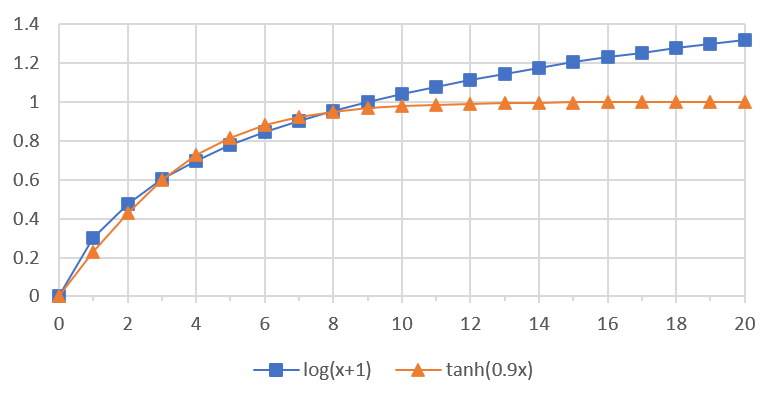
\includegraphics{images/plot_tanh_log.png}}
    \caption{Plot of tanh and log functions}
    \label{fig:plot_tanh_log}
\end{figure}
However, it fails to account for hierarchy effects and economies-of-scale where, as the research staff members increase, they self-organize into a hierarchy, thus reducing the supervision workload on the faculty \parencite{WANG2015197,wellman1997electronic}. We aim to account for this using some non-linearity in the supervision workload. We currently use \(tanh\) due to its closeness to logarithmic functions which tapers off to a maximum (\autoref{fig:plot_tanh_log}), however, more testing is required to arrive at the final definition of the supervision workload, including the weights of research staff types.

\begin{equation}
    \begin{aligned}
        R^s_f & = r\bigg[\frac{2}{(1 + s^{-w} )}- 1\bigg] \\
        w     & = \sum_{r \epsilon R} w_r * n_r           \\
    \end{aligned}
\end{equation}
where,
\begin{equation}
    \nonumber
    \begin{aligned}
        w   & = \text{Sum of total research staff weights} \\
        w_r & = \text{Weight of individual staff type }r   \\
        n_r & = \text{Total number of staff of type }r     \\
        R   & = \text{Set of all staff types}              \\
    \end{aligned}
\end{equation}
\begin{table}[H]
    \centering
    \begin{tabular}{|l|c|c|}
        \hline
        Staff Type         & \(w_r\) \\
        \hline
        Research Assistant & 2       \\
        Post Doc           & 1       \\
        \hline
    \end{tabular}
    \caption{Weights of different research staff types}
\end{table}

Where, \(r\) and \(s\) are parameters defined by the faculty type, to control the behaviour of the function. As an example, for full time professors, we could arrive at \(r=2, s=1.32, R_b = 6 \), thus arriving at the equation below. \autoref{fig:teaching_workload} the plot of the total research workload, for such a distribution  approximated to the nearest \(0.25\) units to make it more realizable.

\[R_f = 6 + 2\bigg[\frac{2}{(1 + 1.32^{-w} )}- 1\bigg]\]

\begin{figure}[H]
    \centering
    \scalebox{0.4}{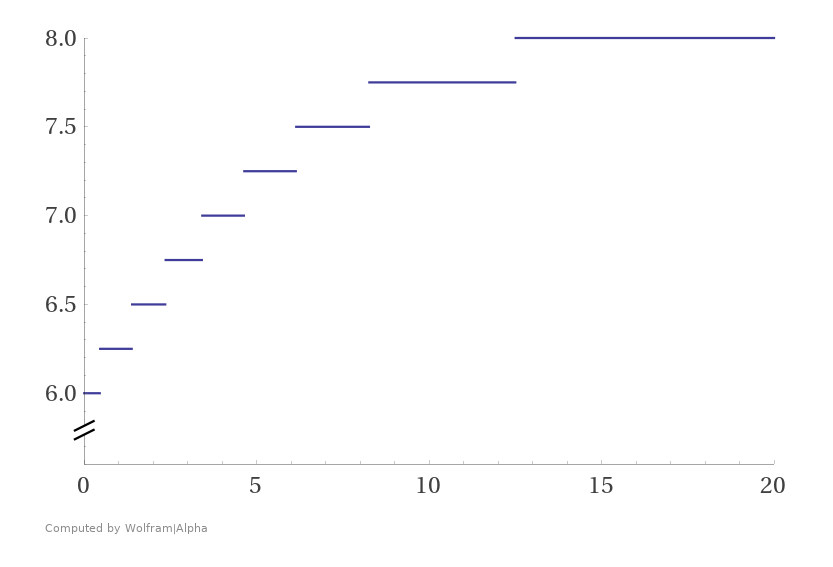
\includegraphics{images/Teaching workload.png}}
    \caption{Teaching Workload}
    \label{fig:teaching_workload}
\end{figure}
\section{Modelling Service Workload}
Service is a challenging part of the workload to measure due to its lack of objectively measurable outputs. In this work, the approach towards quantifying the service workload involves a points system where every service duty \(d\) (like industry attachment officer, course allocation coordinator) corresponds to a set weight \(w_d\). The weighted sum of all the service points will then be normalized to get the service duty workload \(S^d_f\). Similar to the research workload, there will also be a baseline service workload \(S^b_f\) involved to account for faculty-type based service duties (like peer reviews).
\begin{equation}
    \begin{aligned}
        S_f   & = S^b_f + S^d_f                      \\
        S^d_f & = n *\sum_{d\epsilon D}  (w_d * d_f)
    \end{aligned}
\end{equation}
where,
\begin{equation}
    \nonumber
    \begin{aligned}
        w_d & = \text{Weight of the individual service duty }d                    \\
        d_f & = 1\text{, if faculty f carries duty }d\text{, else }0              \\
        n   & = \text{Normalization factor to convert weights into service ratio} \\
        D   & = \text{Set of all service duties}
    \end{aligned}
\end{equation}


However, further exploration is required to list for all the service responsibilities and their corresponding weights. There's also some danger that some service duties cannot be accounted for in this manner, or that certain duties might have different weights faculty to faculty.

\section{Modelling Teaching Workload}
\label{teaching_workload}

Since for a faculty \(f\), the Total Workload \(W_f\) remains fixed, the teaching workload \(T_f\) can be calculated right after the service and research workload has been defined.
\begin{equation}
    \begin{aligned}
        T_f & = W_f - (R_f + S_f)                      \\
        T_f & = 12 - (R^b_f + R^s_f) - (S^b_f + S^d_f)
    \end{aligned}
\end{equation}
As a point of reference and comparison, we define \(T_b\) as the base teaching value for a faculty with no extra Research Supervision and Service Duty workload,  \(R^s_f = S^d_f = 0\). Or simply, \(T^b_f = 12 - R^b_f - S^b_f\). As a shorthand, the ratio of \(R^b_f : T^b_f  : S^b_f\)  for a faculty type will be referred to as the \textbf{RTS ratio}.

\begin{table}[h]
    \centering
    \begin{tabular} { |l |c |c|c|}
        \hline
                  & \(R\) & \(T\) & \(S\) \\
        \hline
        Lecturer  & 2     & 8     & 2     \\
        Professor & 6     & 4     & 2     \\
        \hline
    \end{tabular}
    \caption{RTS Ratio for different faculty types}
    \label{rts_ratio}
\end{table}

Since the total amount of teaching workload (total number of courses taught) remains constant, this teaching ratio is used to calculate the distribution of the fixed teaching workload among all the faculty.


\chapter{Teaching Workload Distribution}
\label{chapter:formal_informal_workload}
% Distributing Teaching Workload

The teaching workload, consisting of formal and informal teaching workload, has some nuances involved in its distribution. This section describes the methodology used for this distribution.

\section{Defining Formal Workload}

\label{section:defining_formal_workload}

Formal Teaching Workload refers to the courses that are taught in a university. A course consists of multiple teaching activities like Lectures, Tutorials and Labs, which need to be quantified. As defined by \parencite{griffith2020framework}, larger classes require more work in non-classroom tasks like grading assignments, office hours etc. A course C can be divided into three sections - the contact hours \(T^c_c\), the administrative work related to the course \(T^a_c\), and the preparatory work \(T^p_c\) .

The preparatory, and contact hours are largely unaffected by class size, while the administrative work heavily depends on the class-size. Course newness and familiarity is something that doesn't affect the contact hours, but has a massive impact on the preparatory work, and has some impact on the administrative work (extra planning and time is required for correction of assignments etc).

For the lecture component, we define the three workloads and the total workload \(T^c\) as

\begin{equation}
\begin{aligned}
	T^c_c &= w*h_w = h  \\
    T^c_p &= h * 3 * n_p \\
    T^c_a &= h * s * n_a \\
    T^c &= T^c_c +T^c_p + T^c_a\\
    T^c &= h(1 + 3 n_p + s*n_a) 
\end{aligned}
\end{equation}
where,
\begin{equation}
\nonumber
	\begin{aligned}
	h_w &= \text{Number of hours of teaching per week}\\
    w &= \text{Number of teaching weeks}\\
    h &= \text{Total number of teaching hours}\\
    s &= \text{Class size factor}\\
    n_a &= \text{Course Novelty Factor - Administration}\\
    n_p &= \text{Course Novelty Factor - Preparation}
   	\end{aligned}
\end{equation}
Tutorials and Labs can only be conducted in fixed-sized groups of about 30-40 each. As a result, although each tutorial/lab session is not affected by the class size directly, the number of sessions increase as the class size increases. Accounting for the rest of the factors of course newness, familiarity etc., we can define the workload of labs and tutorials for every group.

\begin{equation}
\begin{aligned}
	T^c_c &= w*h_w = h  \\
    T^c_p &= h * 3 * n_p \\
    T^c_a &= h * s * n_a \\
    T^c &= T^c_c +T^c_p + T^c_a\\
    T^c &= h(1 + 3 n_p + n_a)
\end{aligned}
\end{equation}

\begin{table}
\centering
\begin{tabular}{|l|l|l|}
	\hline
	Parameter & Constraint & Value \\
    \hline
    \(n_p\) & New to school & 2 \\
     & New to faculty & 1.5 \\
     & Regular & 1 \\
    \hline
    \(n_a\) & New to school & 1.5 \\
     & New to faculty & 1.25 \\
     & Regular & 1 \\
    \hline
\end{tabular}
\caption{Different parameters used in course workload distribution}
\label{course_weightages}
\end{table}

Further exploration and data collection is required to define the exact impact values of the various parameters.

\section{Distributing Formal Workload}
\label{section:distributing_formal_workload}

To distribute the course workload, we use the teaching workload calculated in \autoref{teaching_workload}. However, as seen in \autoref{rts_ratio}, the ratio between lecturers and professors' teaching workload is 2:1. This ratio gets even more skewed as professors get research supervision workload or service duties, which are typically not taken up by lecturers. Thus, in cases of under-supply of faculty expertise, the amount of workload given to lecturers might hit a ceiling, beyond which further work can't possibly be taken up. To resolve this, we allocate in descending order of workload, while a max workload \(C^{max}\) can be given to any given faculty.

To demonstrate, let's take faculty A, B, C, and D, with respective \(T_f\) being 8, 7, 3, and 2. Also, let the total teaching workload be 60 hours and \(C^{max}\) be 20 hours. \(T_{total}= 8+7+3+2 = 20\). So in descending order, Faculty 1 should be given workload \(C_A = 8*60/20=24\), but since 24 > \(C^{max}\), Faculty A will be given \(C_A = 20\). In the same way, B will be given 20. The remainder of workload is equally distributed between C and D as 10 hours each. 

In this way, by using \(C_{max}\), we avoid overloading A and B, by requesting C and D to share the workload of \textbf{10 hours}, instead of the \textbf{6 hours} that they would be originally given.

\section{Distributing Informal Workload}
Informal teaching workload refers to FYPs, Master and PhD students assigned to a faculty. The total informal teaching workload needs to be distributed according to \(T_f\) of the faculty. For this, the total informal teaching workload needs to be distributed among faculties, and then their Masters and PhD workloads subtracted to get the workload available for FYPs. This is because Master and PhD students are typically pre-assigned to the faculty. The exact approach to informal workload distribution, as well as the weekly workload hour impact that each of these three activities, remains to be finalized by looking at the faculty data.

\chapter{Key Factors Affecting Inclusive Teaching Allocation}
\chapter{Key Factors Affecting Inclusive Teaching Allocation}

This section describes the  pre-processing required for teaching allocation, the factors considered in the process, which include considerations for choosing the most appropriate faculty for a course, as well as the constraints that govern the choice. It then goes on to describe the allocation algorithm

\section{Lecture Splitting}
\label{chapter:lecture_splitting}
% Lecture Splitting for Collaborative Teaching

In the interest of distributing workload of large classes, as well as give students more opportunity to find a teaching style that suits them, thus improving understanding and knowledge retention. Collaborative teaching can take many forms, like Parallel teaching, Station Teaching etc \cite{forbes2012successful}. In this work, the strategy of splitting lectures is explored, wherein different lectures are taken by different faculty, which allows accommodation of larger class sizes, as well as improve the equitable distribution of workload. This is approached in a two-step process.

\subsection{Class-size based splitting}
Due to the large class sizes, the amount of administrative teaching work (correcting assignments etc.) can be staggering. Thus, such lectures necessitate splitting to share the workload between, two or more faculty.

\begin{table}
    \centering
    \begin{tabular}{|l|c|}
        \hline
        Class Size             & Split \\
        \hline
        \(<\)250               & 1     \\
        \(\ge\) 250, \(<\) 500 & 2     \\
        \(\ge\) 500            & 3     \\
        \hline
    \end{tabular}
    \caption{Class-size based splitting}
    \label{class_size_splitting}
\end{table}

The tutorials sessions are always split into groups of \(< 40\) each and different may be taken up by different faculty as the need arises.

\subsection{Post-Allocation Splitting}
During the allocation phase, inequity is likely to take place due to varying fields that the faculties have expertise in. The post-allocation splitting aims primarily at solving this problem. This splitting takes place only after the initial course-workload allocation between faculties has already taken place.

Given that quality of allocations is not notably sacrificed, and class-size meets a minimum size \(S_{min}\), splitting courses is attempted such that on high-utilization and medium-utilization faculty such that -

\begin{enumerate}
    \item Under-utilized faculty can serve high-utilization faculty’s courses
    \item Under-utilized faculty can serve medium-utilization faculty’s courses
    \item Medium-utilized faculty can serve high-utilization faculty’s courses
\end{enumerate}

Further work is required to clearly define the thresholds that delineate high, medium and low utilization, as well as \(S_{min}\) suitable for such splitting. Further experiments and data analysis on existing courses also needs to be done to test if this technique yields positive results.

% Teaching Allocation Criteria

% \item \textbf{Faculty-wise lecture, labs and tutorials workload weightages}

% These refer to teaching activities involved in the courses, expressed in hours. The lectures, labs and tutorials are weighted according to class-size, course novelty factors etc (Static Lecture Weightage). After this, additional weightage is given to individual faculty's familiarity to the courses (Dynamic Weightage).

% \item \textbf{Faculty-Course Match Rating}

% This is a combination of the faculty's teaching performance in individual courses, along with their preferences and the course priority. The teaching performance takes the highest precedence, with the course priority skewing the data in such a way as to favour allocation of important courses to faculty with good feedback in said courses. The preferences come into play when the available faculty are on a level-playing field and one is not drastically better than the other.

\section{Allocating Suitable Faculty}
\label{section:allocation_criteria}

There are multiple factors that need to be considered while choosing the faculty to be allocated for a course,
\subsection{Course Priority}
Certain courses require a lot more attention than other courses. The reasons can be an attribute of the students studying in the course, or the contents of the course themselves. Some considerations into the priority of courses are
\begin{enumerate}
    \item \textbf{Seniority of students} - Courses of lower years require more attention, as newly on-boarded students may not be well acquainted with the university teaching styles and pressures.
    \item \textbf{Foundational Courses} - Certain courses form the foundation for many courses later in the students' academic journeys. Foundations of programming and algorithm design are core skills that a computer science engineer could require, for example. Thus, special attention needs to be paid to account for such courses.
    \item \textbf{Course Difficulty} - Tougher courses generally require more teaching expertise.
\end{enumerate}

\subsection{Faculty Preferences}
A key factor that governs faculty satisfaction is the ability to choose their courses and teaching areas \cite{schniederjans1987goal, badri1998multi}. This allows the faculty to align their research to the courses they teach, discover new opinions in their areas of expertise, etc. while avoiding courses they feel are largely irrelevant to their career path and interests. On top of this, the ability to specify their schedule preferences, like being able to condense their teaching hours into certain days of the week, etc. allows them to focus much better on their research. An allocation system should, thus, be able to account for such preferences.

\subsection{Faculty Performance}
Different faculty have different areas of excellence. Some faculties are more research intensive, others are great teachers, while others are gifted in administrative and management roles. However, teaching performance is important, especially in aforementioned high-priority courses, and thus needs to be accounted for. Student and peer feedback ratings are a reliable indicator of the teaching quality that can be used into this effect.

\section{Allocation Constraints}

The allocation algorithm operates under certain hard and soft constraints that need to be honoured. Hard constraints being the constraints that cannot be violated, while soft constraints being the constraints that have to be honoured as long as feasible, but can be ignored in odd circumstances.

The constraints are as follows:
\begin{enumerate}
    \item \textbf{Teaching Workload Weightage} (Soft)

          After the teaching workload is calculated as an output of the workload model, this weightage is used to distribute the amount of formal teaching workload to be allocated to each faculty. This workload weightage should never be violated, unless, there are courses that will go unallocated if not assigned to aforementioned faculty.

    \item \textbf{Maximum Teaching Capacity} (Hard)

          Faculty (primarily lecturers) should never be assigned teaching workload beyond the max capacity defined in the system. This is because the capacity is defined with the absolute maximum feasibility in mind and, if exceeded, could lead to a drastic reduction in teaching quality due to deal with course related preparatory work/administrative duties.

    \item \textbf{Non-Preferred Courses} (Soft)

          Courses low on the faculty preference list should generally not be allocated, unless no other viable faculty is available.

    \item \textbf{Courses without expertise} (Hard)

          A faculty cannot teach a course they don't have any expertise in. In practical terms, this means that courses the faculty hasn't previously taught, or aren't anywhere in their preference list, should not be allocated to the faculty.

    \item \textbf{Faculty isn't given too many courses} (Soft)

          The faculty workload should be concentrated into as few courses as possible, due to the additional work required in course preparation for every additional course. In practical terms, this means tutorials/lab of a course should ideally be allocated to the same faculty that takes up the lectures.

    \item \textbf{Equal distribution of various teaching activities} (Soft)

          Each faculty should ideally receive an equal ratio of tutorials/labs/lectures to other faculty. This means that a faculty shouldn't for example, receive a disproportionate number of tutorials as this would require a lot of preparation work and will stagger their work hours too much.
\end{enumerate}
\section{Allocation Algorithm}

These inputs and constraints are then passed to the allocation engine/algorithm. The algorithm will either operate sequentially (goal-programming/greedy methods), in which case the outputs can be used to feedback to the faculty-course matcher and improve allocation quality and better account for the faculty's utilization, or it can operate parallelly (many-to-many Munkres algorithm), in which case such a feedback cycle isn't possible. There is also some possibility that the algorithm could operate in multiple sequential stages of parallel allocation, with different levels of priority courses being allocated at different stages. Further work is required to specify the exact details of this algorithm.


\chapter{Framework for Workload-Aware Teaching Allocation}
%  Integrated Framework for Faculty Workload Aware Teaching Allocation

This section describes how the different areas of research come together to define the allocation framework. It goes on to present a diagram of the framework in \autoref{fig:system_architecture}.

\section{Formal Teaching Workload Allocation}

Formal Teaching Workload allocation refers to allocation of courses, tutorials and labs to individual faculty while keeping their preferences and constraints in mind.

\subsection{Teaching Workload Weightage Calculator}

This involves using the findings in \autoref{chapter:rts_ratio} and \autoref{section:distributing_formal_workload} to calculate the teaching workload that should to be allocated to a faculty, while taking into account the faculty's role, their research and service duties, while also keeping in mind the max workload that can be allocated to a faculty due to practical considerations.

\subsection{Lecture Splitter}

This involves applying the insights from \autoref{chapter:lecture_splitting} into splitting the lectures on the basis of class size and other factors, with the aim of distributing the workload equitably while also keeping the impact of one particular course on a faculty low.

\subsection{Course Weightage Calculator}

This involves applying the insights and calculation methodology from \autoref{section:defining_formal_workload} to calculate the weightages for lectures, tutorials and labs of each course while making considerations for class size, course newness and faculty-course familiarity which affect the amount of work required for them. 

\subsection{Faculty Course Matcher}

This involves applying the factors described in \autoref{section:allocation_criteria} to define the most appropriate faculty for a course and condensing these factors into weightages that can be directly used to by the allocation algorithm. Studies have pointed to the biases that student feedback suffers from, including language, accent, racial and gender preferences. However, not all such biases hold true in rating a faculty's teaching capability. In an attempt to solve this, finding methods to counter such biases is an area that will be explored.

\subsection{Allocation Engine}

This involves using the allocation algorithm taking the inputs provided by the Course Weightage Calculator to allocate the courses on the basis of appropriateness defined by the Faculty Course Matcher, and also meeting the constraints defined by the Teaching Workload Weightage Calculator to allocate the courses to faculty while maintaining an optimal and equitable distribution of workload for the faculty.

\section{Informal Teaching Workload Allocation}

Informal Teaching Workload Allocation refers to allocation of FYPs for the faculty on the basis of the workload constraints defined in the Teaching Workload Weightage Calculator, and also taking into consideration the number of Masters' and PhD students under the individual faculty.

\section{Management Insights}

Management Insights gathers statistical insights provided by all the above modules to describe the overall allocation quality in factors such as-
\begin{itemize}
\item Fulfilment of organizational goals
\item Equity and outliers in the workload distribution of faculty
\item Gaps in faculty expertise which result in aforementioned outliers
\item Overdependence on certain faculty members
\end{itemize}

\section{Framework diagram and Research Timeline}

The diagram gives a high-level view of the submodules, inputs, and outputs of the allocation framework. The diagram after describes the timeline for completion of the research.

\begin{sidewaysfigure}
	\centering
    \scalebox{.16}{\includegraphics{images/overview.png}}
    \caption{Overview of the system architecture}
    \label{fig:system_architecture}
\end{sidewaysfigure}

\begin{sidewaysfigure}
    \centering
    \scalebox{0.9}{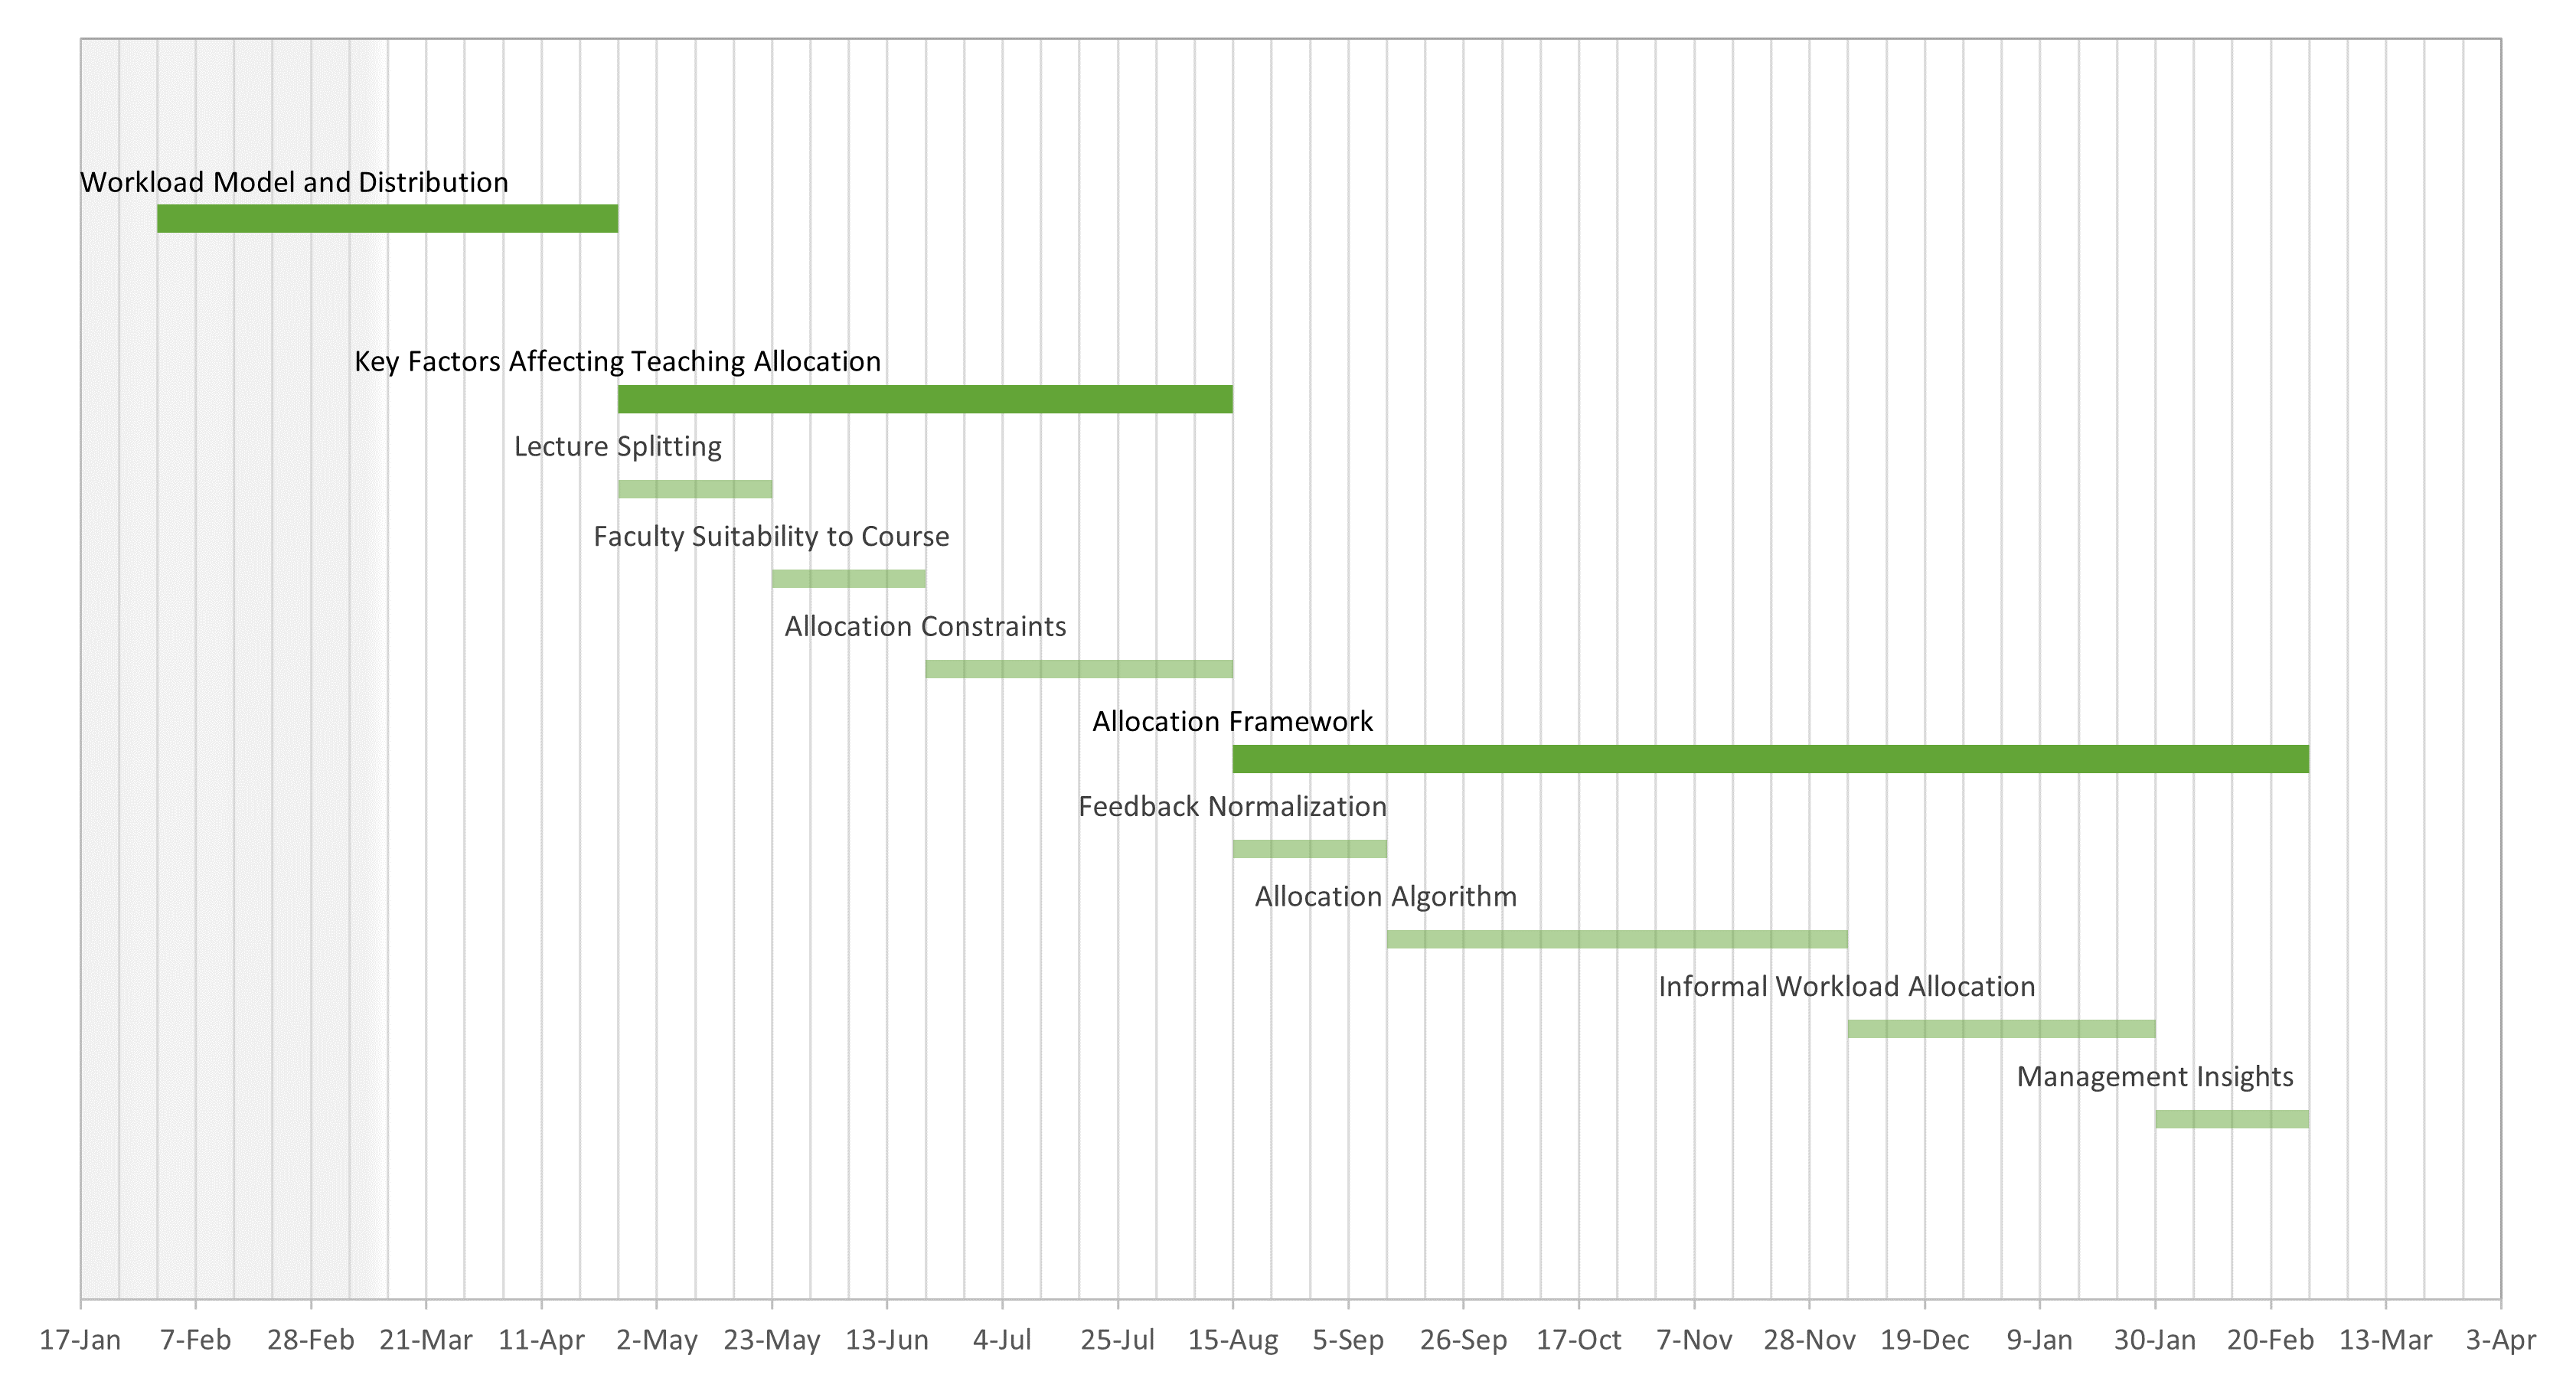
\includegraphics{images/gantt_chart.png}}
    \caption{Research Timeline plan}
    \label{fig:gantt_chart}
\end{sidewaysfigure}


\chapter{Further Work and Timeline}
\chapter{Conclusion and Future Work}

\section{Conclusion}

In this thesis, the problem of automated teaching workload allocation to faculty members was addressed. The proposed solutions were found to be holistic and effective, and were able to allocate all teaching workload to the faculty, while ensuring that the allocation was fair and equitable, and prioritized the student feedback, the faculty preferences, and the management priorities.

To allocate the courses, the problem was split into four sub-problems - the quantification of the workload involved in the teaching activities of a course, determining how much workload each faculty member should be assigned, allocating lectures to the faculty members, and allocating tutorials and lab sessions to the faculty members.

To quantify the workload involved in the teaching activities of a course, the activity was divided into four distinct stages, namely - preparation, review, delivery, and grading Workload. The preparation workload and grading workload were only applicable to the course lecturer, while the review workload and delivery workload applied to all faculty members involved in the teaching of the course. For each of these stages, the factors affecting the workload were identified. The factors were the course newness, class size, and activity type (lecture, tutorial, or lab). Using these factors, a model was developed to quantify the workload involved in the three teaching activities of the course in the form of Workload Units. The model was found to be effective and was able to quantify the workload of the teaching activities accurately and comprehensively in a variety of scenarios.

The workload of tutorials and lab sessions was found to be typically 20-40 units. It was found that the workload of a lecture can range anywhere from 80 to 600 units, being higher for larger class sizes, and if the course is being taught for the first time. The high workload of a lecture would result in difficulties finding eligible faculty to teach the lecture without overloading them. To alleviate this, a lecture splitting algorithm was developed, that splits the workload of a lecture into 2-3 smaller lectures, which can be allocated to multiple faculty members. The lecture-splitting algorithm was found to be effective in reducing the workload of high-workload lectures and was able to reduce the overloading of faculty.

To determine how much workload each faculty member should be assigned, the research and service workload of the faculty were quantified. The research workload was quantified in terms of the number of research staff that the faculty is supervising, while the service workload was quantified in terms of the service duties that the faculty is performing.

The workload was then modeled into an RTS ratio, to represent the Research, Service, and Teaching workload, the sum of the three components always being 12 since the total workload of each faculty is comparable. The RTS ratio was found to be a good representation of the workload of the faculty. The RTS ratio was then used to determine the $T$ ratio, by subtracting the research and service workload from the total workload of the faculty i..e 12. This $T$ ratio is the teaching workload that should be allocated to the faculty in relative terms.

To allocate lectures to the faculty members, the Hungarian Algorithm was used, which allocates one lecture per faculty member in every iteration. The $T$ ratio of the faculty, combined with the workload of the lecture, was used to determine the workload limit for the faculty, which was used to ensure that the faculty members were not overloaded with work.

It was found that lectures remained unallocated in certain cases, due to various reasons. In one case, \textbf{44\%} of the lectures remained unallocated. To handle this, various techniques were developed. These techniques were pre-allocating lectures with supply shortages, dynamic-splitting unallocated lectures into two smaller lectures to allocate to faculty, workload-limit-relaxation to allow for overloading of faculty, and Dynamic Swapping to free up some faculty who can teach the remaining unallocated lectures. As a result of these techniques, up to \textbf{98\%} of the lectures were allocated to the faculty. As a final step, an equal misery approach was devised, which allowed up to \textbf{99\% of the lectures to be allocated} to the faculty.

Similar techniques were used for the allocation of tutorials, with some changes to allocate one tutorial session per faculty in every iteration to allow the same faculty to teach multiple sessions of the same course tutorial. However, it was found that on average, a course had \textbf{4.5 different faculty teaching the tutorials of the course}. To avoid reducing this fragmentation, batching of tutorials into groups of up to 6 tutorials of the same course, and adding a consistency bias were introduced. These measures were found to be very effective and reduced the number of faculty teaching the tutorials of the same course to \textbf{1.2 faculty per course}.

Additionally, pre-allocation of tutorials was also implemented, similar to lecture pre-allocation, which was able to improve tutorial allocation by an additional 3\%, from 73\% to 76\%. Workload relaxation was avoided, in favor of a dynamic limit adjustment approach which is more targeted. The dynamic limit adjustment approach was found to be very effective and was able to \textbf{improve tutorial allocation from 76\% to 100\%}, allocating all tutorials to the faculty, without adversely affecting the workload limits of the faculty.

The allocation of labs was identical to tutorial allocation and with the combination of pre-allocation, dynamic limit adjustment, consistency bias, and all the other techniques, \textbf{100\% of the lab sessions were allocated to the faculty, with an average of 1.4 faculty teaching the labs of the same course}.

With the allocation of all teaching activities to the faculty using the Hungarian Algorithm, incorporating the RTS ratio and measuring the workload impact of the teaching activities, an allocation was achieved that was fair and equitable while prioritizing the student feedback, the faculty preferences, and the management priorities.

\section{Future Work}

The allocation of teaching workload to faculty is a complex problem, and while the allocation achieved in this thesis is fair and equitable, there are still certain areas of improvement that can be made. Some of these areas are discussed below.

\subsection{Workload Analysis from the RTS Model}

The RTS Model provides a lot of insight into the workload of the faculty and can be used to derive important metrics regarding the health of the institution. It can be used to determine if the overall organizational objectives of the institution are met, by ensuring that the aggregate RTS ratio of the institution is in the right direction. A research-intensive university may aim for an aggregate RTS Ratio of $R:T:S = 6:4:2$, for example.

It can also be used to determine if the faculty are overloaded with work, by checking if the RTS ratio corresponds to the actual workload self-reported by the faculty. A misalignment between the two can indicate that the faculty are overloaded with work, and can be used to determine if additional faculty need to be hired.

\subsection{Better prioritization of earlier year courses}

Many techniques such as pre-allocation, dynamic splitting, and workload relaxation, needed to be developed to overcome unallocated lectures which were a result of absolute prioritization of earlier year courses. Primitive analysis of allocating all years together showed that many of the unallocated lectures would be allocated if the lectures weren't allocated year-wise. However as shown in tutorial allocation, a year-wise bias was not very effective.

If a better way of prioritizing earlier-year courses can be found, it would be possible to allocate all lectures together, instead of allocating lectures year-wise, which could yield better results. This can be explored in future work.

\subsection{Prioritization of Foundational Courses}

Certain courses are considered to be foundational courses, which are important for the students to learn, and are also important for the students to perform well in, as they are prerequisites for other courses, and play an important part in the students' learning journey. Allocating earlier-year courses to the best faculty broadly serves to prioritize such foundational courses, but it is not very targeted.

An analysis of course prerequisites can be performed, to determine which courses are foundational, and can be given a higher priority in the allocation process. Exploring these interdependencies, such as analyzing the effect of student performance in a foundational course on the student performance in the subsequent courses, can highlight other valuable insights, that can be used to improve the allocation process and learning outcomes for the students.

\subsection{Prioritizing Faculty with Prior Experience in the Course}

As shown in the course workload model, faculty who have previously taught a course have a lower workload than faculty who are teaching the course for the first time. Thus, prioritizing faculty who have previously taught a course can be an additional consideration in avoiding the fragmentation of tutorials and labs. This can also be incorporated into lecture allocation, as it has the potential of lowering overall teaching workload in the institution, and can be explored further.

Additionally, the reduction of workload accompanied by teaching multiple tutorials of the same course is not accounted for in the current model and can be incorporated into the model in future work.

\subsection{Timetabling Constraints}

Timetabling of the courses is carried out separately, independent of the allocation of teaching workload to faculty. However, the two processes are interdependent, and if two courses are timetabled at the same time, they cannot be taught by the same faculty. This can be incorporated into the allocation process, to ensure that the courses are timetabled in a way that allows the courses to be taught by the same faculty.

Other timetabling constraints like the distance between classrooms can also be incorporated into the allocation process, to ensure that faculty have adequate time to reach the classroom after teaching another class. This can be explored in future work.

\subsection{Workforce Gap Analysis}

Techniques like pre-allocation highlighted the shortage of eligible faculty for certain courses. This can be used to perform a workforce gap analysis, which can be used to determine the number of additional faculty that need to be hired to ensure that all courses can be taught by eligible faculty. This, in combination with the need for systematic overloading of faculty, shows the possibility for a more targeted hiring process, which can be beneficial for the institution.


% Include appendix      % Set this up if needed
%\appendix

\singlespacing
% Insert bibliography here
\printbibliography


\end{document}

% End of document
%-----------------------------------------------------------------------------------------------------
